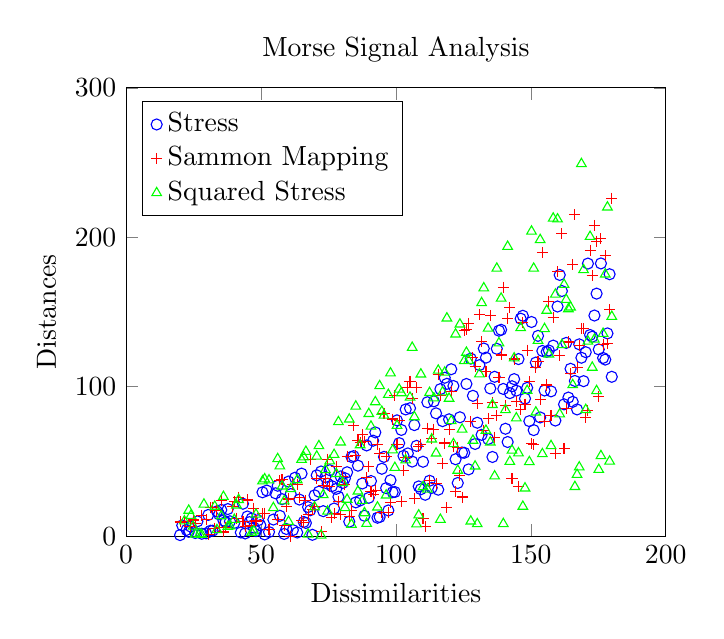
\begin{tikzpicture}
\begin{axis}[
  only marks,                    % no lines
  xmin=0, xmax=200,              % x-axis limits
  ymin=0, ymax=300,              % y-axis limits
  xlabel={Dissimilarities},      % x-axis label
  ylabel={Distances},            % y-axis label
  title={Morse Signal Analysis}, % plot title
  legend pos=north west,         % legend position on plot
  legend cell align=left,        % text alignment within legend
  domain=20:180,                 % domain for plotted functions (not needed for scatter data)
  samples=200,                   % plot 200 samples
]
  \addplot[mark=o,blue] {x^2/200 + rand*x/3}; % add the first plot
  \addlegendentry{Stress}; 					  % add the first plot's legend entry
  \addplot[mark=+,red]  {x^2/200 + rand*x/2};
  \addlegendentry{Sammon Mapping};
  \addplot[mark=triangle,green] {x^2/200 + rand*x/1.5};
  \addlegendentry{Squared Stress};
\end{axis}
\end{tikzpicture}